\documentclass{beamer}
\usepackage[utf8]{inputenc}
\usepackage{comment}
\usepackage[maxbibnames=99]{biblatex}
\definecolor{cvut_navy}{HTML}{0065BD}
\definecolor{cvut_blue}{HTML}{6AADE4}
\definecolor{cvut_gray}{HTML}{156570}
\definecolor{faeng_blue}{HTML}{09246F}
\usepackage[makeroom]{cancel}
\usepackage{threeparttable}

\setbeamercolor{section in toc}{fg=black,bg=yellow}
\setbeamercolor{alerted text}{fg=cvut_blue}
\usepackage{tikzsymbols}
\usepackage{textcomp}
\usepackage{parskip}
\definecolor{darkblue}{rgb}{0, 0, 0.5}
\definecolor{babyblue}{rgb}{0.54, 0.81, 0.94}
\usepackage{pgf}
\usepackage{color,soul}
\usepackage{tcolorbox}
\tcbuselibrary{skins}
\usepackage{minted}
\usepackage{hyperref}
\usepackage{xcolor,soul}
\definecolor{lightblue}{rgb}{.90,.95,1}
\sethlcolor{lightblue}

\renewcommand<>{\hl}[1]{\only#2{\beameroriginal{\hl}}{#1}}
\setbeamertemplate{page number in head/foot}[totalframenumber]

\usepackage{empheq}
\usepackage{xcolor}
\definecolor{lightgreen}{HTML}{90EE90}
\newcommand{\boxedeq}[2]{\begin{empheq}[box={\fboxsep=6pt\fbox}]{align}\label{#1}#2\end{empheq}}
\newcommand{\coloredeq}[2]{\begin{empheq}[box=\colorbox{lightgreen}]{align}\label{#1}#2\end{empheq}}
\newcommand{\highlight}[1]{\colorbox{red!40}{$\displaystyle#1$}}

\definecolor{babyblue}{rgb}{0.54, 0.81, 0.94}
\definecolor{babypink}{rgb}{0.96, 0.76, 0.76}
\definecolor{blue(ncs)}{rgb}{0.0, 0.53, 0.74}
\definecolor{pistachio}{rgb}{0.58, 0.77, 0.45}
\definecolor{darksalmon}{rgb}{0.91, 0.59, 0.48}
\definecolor{lightsalmonpink}{rgb}{1.0, 0.6, 0.6}
\definecolor{columbiablue}{rgb}{0.61, 0.87, 1.0}
\definecolor{corn}{rgb}{0.98, 0.93, 0.36}
\definecolor{jonquil}{rgb}{0.98, 0.85, 0.37}
\definecolor{bananayellow}{rgb}{1.0, 0.88, 0.21}
\newcommand{\bert}{\ensuremath{
    \mathchoice{\includegraphics[height=2ex]{Bert-pic-removebg-preview.png}}
        {\includegraphics[height=2ex]{Bert-pic-removebg-preview.png}}
        {\includegraphics[height=1.5ex]{Bert-pic-removebg-preview.png}}
        {\includegraphics[height=1ex]{Bert-pic-removebg-preview.png}}
}}

\useoutertheme{infolines}

\usepackage{courier}
\usepackage{expl3}
%\usepackage[listings,theorems]{tcolorbox}

\newcommand\scroll[4][§§]{
  \seq_set_split:Nnn\g_inputline_seq{#1}{#4}
  \seq_map_inline:Nn\g_inputline_seq{
    \seq_gput_right:Nx\g_linebuffer_seq{##1}
    \int_compare:nT{\seq_count:N\g_linebuffer_seq>#3}{
      \seq_gpop_left:NN\g_linebuffer_seq\dummy
    }
  }
  \fbox{\begin{minipage}[t][#3\baselineskip]{#2}
    \ttfamily
    \seq_map_inline:Nn\g_linebuffer_seq{\mbox{##1}\\}
  \end{minipage}}
}
\newcommand\clearbuf{\seq_gclear:N\g_linebuffer_seq}
\ExplSyntaxOff

\setbeamertemplate{headline}{%
\begin{beamercolorbox}[colsep=1.5pt]{upper separation line head}
\end{beamercolorbox}
\begin{beamercolorbox}{section in head/foot}
    \vskip2pt\insertsectionnavigationhorizontal{\paperwidth}{}{\hskip0pt plus1filll}\vskip2pt
\end{beamercolorbox}%

\begin{beamercolorbox}[colsep=1.5pt]{lower separation line head}
\end{beamercolorbox}
}
\makeatletter
\newcommand\SoulColor{
  \let\set@color\beamerorig@set@color
  \let\reset@color\beamerorig@reset@color}
\makeatother
\SoulColor
\usepackage{amsmath, bm}
\usepackage{tikz}
\setbeamercovered{dynamic}

\newcommand{\highlightt}[1]{%
  \colorbox{blue!40}{$\displaystyle#1$}}

\newenvironment<>{problock}[1]{%
    \begin{actionenv}#2%
        \def\insertblocktitle{#1}%
        \par%
        \mode<presentation>{%
        % \setbeamercolor{block title}{fg=white,bg=orange!20!black}
          %\setbeamercolor{block title}{fg=white,bg=red!10!black}
          \setbeamercolor{block title}{fg=white,bg=babyblue}
        \setbeamercolor{block body}{fg=black,bg=white!50}
        \setbeamercolor{itemize item}{fg=orange!20!black}
        \setbeamertemplate{itemize item}[triangle]
      }%
        \usebeamertemplate{block begin}
      \par\usebeamertemplate{block end}
      \end{actionenv}
      }

      \newcommand<>{\uncovergraphics}[2][{}]{
      % Taken from: <https://tex.stackexchange.com/a/354033/95423>
      \begin{tikzpicture}
      \node[anchor=south west,inner sep=0] (B) at (4,0)
          {\includegraphics[#1]{#2}};
      \alt#3{}{%
          \fill [draw=none, fill=background, fill opacity=0.9] (B.north west) -- (B.north east) -- (B.south east) -- (B.south west) -- (B.north west) -- cycle;
      }
      \end{tikzpicture}
}

\newlength\dlf
\newcommand\alignedbox[3][yellow]{
    % #1 = color (optional, defaults to yellow)
    % #2 = before alignment
    % #3 = after alignment
    &
    \begingroup
    \settowidth\dlf{$\displaystyle #2$}
    \addtolength\dlf{\fboxsep+\fboxrule}
    \hspace{-\dlf}
    \fcolorbox{red}{#1}{$\displaystyle #2 #3$}
    \endgroup
}

\usepackage{collcell}
%\usepackage{remreset}% tiny package containing just the \@removefromreset command
\makeatletter

\usepackage{xcoffins}
\NewCoffin\tablecoffin
\NewDocumentCommand\Vcentre{m}
  {%
    \SetHorizontalCoffin\tablecoffin{#1}%
    \TypesetCoffin\tablecoffin[l,vc]%
  }

\usepackage{pgfpages}
\graphicspath{{images/}}

%% Important
%%% show note or disable note.
%\setbeameroption{show notes on second screen=right} % Both

\setbeamertemplate{note page}{\pagecolor{gray!5}\insertnote}\usepackage{palatino}
\usepackage{xcolor}
\usepackage{soul}
\usepackage{etoolbox}
\makeatletter
%\patchcmd{\slideentry}{\ifnum#2>0}{\ifnum2>0}{}{\@error{unable to patch}}% replace the subsection number test with a test that always returns true
\makeatother

%\setbeamercolor*{palette primary}{bg=cvut_navy,fg=gray!20!white}
\setbeamercolor*{palette primary}{bg=faeng_blue,fg=gray!20!white}
\setbeamercolor*{palette secondary}{bg=faeng_blue,fg=gray!20!white} % no color
%\setbeamercolor*{palette secondary}{bg=cvut_navy,fg=cvut_navy}
%\setbeamercolor*{palette secondary}{bg=cvut_blue,fg=white}
\setbeamercolor*{palette tertiary}{parent=palette primary} % color of the top and date
\setbeamercolor*{palette quaternary}{fg=faeng_blue,bg=gray!5!white}
\setbeamercolor*{sidebar}{fg=faeng_blue,bg=gray!15!white}
\usepackage[first=0,last=9]{lcg}
\usepackage{color, colortbl}
\usepackage{stackengine,tikz}
\usepackage{transparent}
\colorlet{Gray}{gray!30}
\newcommand*{\MinNumber}{0}%
\newcommand*{\MaxNumber}{0.4}%
\definecolor{bubblegum}{rgb}{0.99, 0.76, 0.8}
\newcommand{\ApplyGradient}[1]{%
  \pgfmathsetmacro{\PercentColor}{100.0*(#1-\MinNumber)/(\MaxNumber-\MinNumber)}%
  \edef\x{\noexpand\cellcolor{babyblue!\PercentColor}}\x\textcolor{black}{#1}%
}
\newcolumntype{R}{>{\collectcell\ApplyGradient}{c}<{\endcollectcell}}

\setbeamercolor{titlelike}{parent=palette primary}
\setbeamercolor{frametitle}{parent=palette primary}

\setbeamercolor{B}{bg=red!30,fg=black}

\setbeamertemplate{section in toc}[default]
\setbeamercolor{itemize item }{fg=blue}
\setbeamertemplate{itemize item}[circle]

\setbeamercolor*{separation line}{}
\setbeamercolor*{fine separation line}{}

\setbeamertemplate{navigation symbols}{}
\setbeamertemplate{caption}{\raggedright\insertcaption\par}

\setbeamercolor*{block title example}{fg=white,bg=purple!75!black}
\setbeamercolor*{block body example}{fg= black, bg= white}

\setbeamercolor{itemize item}{fg=cvut_navy} % all frames will have red bullets
\setbeamercolor{block title}{bg=red!30,fg=black}
\setbeamertemplate{subsection in toc}[subsections numbered]

\usepackage{eqnarray,amsmath}
\usepackage{amsfonts}
\usepackage{amssymb}
\usefonttheme{professionalfonts}
\usepackage{graphicx}
\usepackage{booktabs}
\usepackage{bm}
\usepackage{mathtools}
\usepackage[utf8]{inputenc}
\usepackage[T1]{fontenc}
\usepackage[russian]{babel}
\usepackage{lmodern}

\setbeamercolor{block title}{fg=black, bg=yellow}
\setbeamercolor{block2}{use=structure,fg=white,bg=purple!75!black}

\def\bq{\mbox{\kern.1ex\protect\raisebox{-1.3ex}[0pt][0pt]{''}\kern-.1ex}}
\def\eq{\mbox{\kern-.1ex``\kern.1ex}}
\def\ifundefined#1{\expandafter\ifx\csname#1\endcsname\relax }%
\ifundefined{uv}%
        \gdef\uv#1{\bq #1\eq}
\fi

\usepackage{algpseudocode}
\usepackage{ragged2e}
\usepackage{csquotes}

\usepackage{biblatex}
\addbibresource{referencias.bib}


%====================================================
%========== DEFINITION OF AUTHORS ETC...=============
%====================================================

\author[Глаз Роман Сергеевич]{Политика регулирования частот центрального процессора в ядре Linux для приложений реального времени
    \\ \vspace{2mm} Глаз Роман Сергеевич}
\institute[]{

    Московский физико-технический институт  \\
    Кафедра микропроцессорных технологий в интеллектуальных системах управления
    \vspace{1mm} \\
    % \textbf{Научный руководитель:}  \\
    % Кринов Пётр Сергеевич, к. ф.-м. н.
}

\title[]{Выпускная квалификационная работа бакалавра}
% \title[]{Политика регулирования частот центрального процессора в ядре Linux для приложений реального времени}

\date[\today]{\small{} \\ \small{\today}}

%====================================================
%========== BEGINNING OF DOCUMENT ===================
%====================================================

\begin{document}

\begin{frame}[plain]
	\titlepage
	\begin{center}%
  		\includegraphics[height=1.3cm]{images/mipt_logo.png}
	\end{center}
\end{frame}

% =========================================

\section{Введение}

\begin{frame}{Актуальность}
    \begin{enumerate}
      \item Производительность современных ЦП ограничена производительностью системы памяти.
      \item Память: несколько уровней кешей и ОЗУ.
      \item Современные операционные системы (Linux, FreeBSD) не учитывают задержки памяти при регулировании
          тактовых частот ЦП и планировании задач, из-за чего возможен неоправданный рост
          тактовых частот и энергопотребления.
      \item Для приложений реального времени важно избегать деградации производительности
        при возможном наименьшем энергопотреблении ядер ЦП.
    \end{enumerate}
\end{frame}

\begin{frame}{Пример организации памяти}
    \begin{figure}
        \centering
        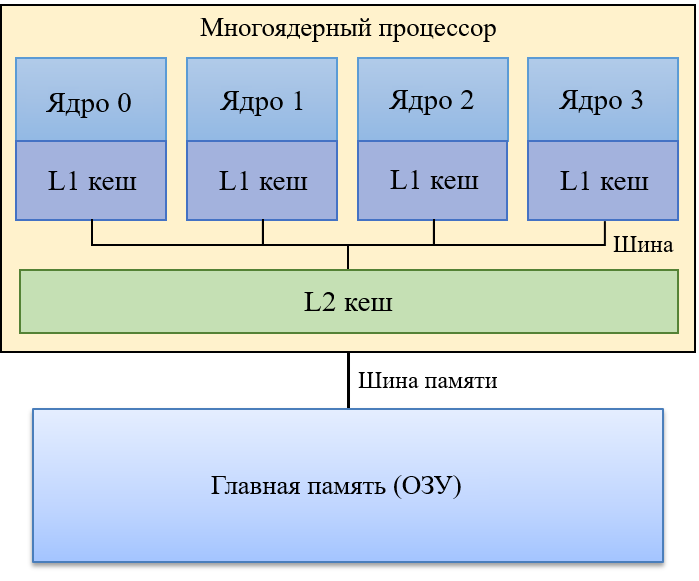
\includegraphics[width=6.8cm]{MulticoreCacheRU.png}
        \caption{Пример организации памяти в устройстве с многоядерным ЦП}
        \label{pic:cache_pyramid}
    \end{figure}
\end{frame}

% =========================================

\section{Цели и задачи}

\begin{frame}{Цели работы}
    \begin{enumerate}
    %   \item Разработать механизмы для сбора статистики микроархитектурных
    %       событий ядер ЦП при различных тактовых частотах для устройств эмулятора Gem5.
    % \item Gem5 -- эмулятор компьютерных архитектур с открытым исходным кодом,
    % позволяющий запускать ОС Linux.
      \item Разработать модель производительности ядер ЦП с учётом поведения и характеристик
          устройств памяти (кеши ЦП, ОЗУ).
      \item Разработать способ применения модели в ядре операционной системы Linux,
      реализовать политику регулирования частот ядер ЦП.
    \end{enumerate}
\end{frame}

\begin{frame}{Задачи}
    \begin{enumerate}
        \item Реализовать в ядре операционной системе Linux (версии 6.1):
        \begin{enumerate}
            \item Набор драйверов, позволяющих изменять тактовые частоты ЦП в эмулируемой системе
                архитектурным симулятором Gem5.
            \item Возможность сбора статистики микроархитектурных событий ядер ЦП, связанных с работой
                кешей, для архитектуры ARM64.
        \end{enumerate}
        \item Разработать модель производительности ядер ЦП:
        \begin{enumerate}
            \item Спроектировать теоретическую модель производительности ЦП.
            \item Реализовать набор бенчмарков, подходящих для построенной модели, и собрать для них
                статистику микроархитектурных событий при различных частотах ЦП.
            \item Найти коэффициенты модели на основе снятых данных.
        \end{enumerate}
        \item Реализовать политику регулирования тактовых частот ядер ЦП в ядре Linux,
            используя разработанную модель.
    \end{enumerate}
\end{frame}

% =========================================

\section{Обзор существующих решений}

\begin{frame}{Обзор существующих решений}
    \begin{enumerate}
        \item В ядре Linux неявным образом предполагается линейная зависимость производительности
        ядра процессора от его тактовой частоты:
        \begin{enumerate}
            \item В подсчёте утилизации потоков исполнения и ядра ЦП.
            \item В регулировании тактовых частот ядер ЦП, в том числе
            на основе подсчитанной утилизации.
        \end{enumerate}
        \item Существует ряд альтернативных моделей производительности ЦП, которые, как правило:
        \begin{enumerate}
            \item Используют данные, которые нельзя получить в режиме реального времени.
            \item Не учитывают наличие возможности регулирования тактовых частот ЦП.
            \item Применимы только для конкретных приложений (отсутствует обобщение).
        \end{enumerate}
    \end{enumerate}
\end{frame}

% =========================================

\section{Исследование}

\begin{frame}{Исследование и построение решения}
    Построена следующая теоретическая модель производительности (для системы с 3-мя уровнями кешей):
    \begin{equation}
        cpi = cpi_{L1/L2} + \alpha_{mem}^{par} \cdot
        \left( \beta_1 \cdot (l2pi - l3pi) + \beta_2 \cdot l3pi \right) \cdot freq_{cpu}
    \end{equation}
    \begin{enumerate}
        \vspace{-3mm}
        \item $cpi$ -- количество затраченных тактов на инструкцию.
        % \item $cpi_{L1/L2}$ -- часть $cpi$, не связанная с обращениями в кеш 3-его уровня и ОЗУ.
        \item $l2pi$ и $l3pi$ -- количество промахов в кеши 2-ого и 3-ого уровней на единицу инструкции.
        \item $freq_{cpu}$ -- тактовая частота ядра процессора.
        \item $\alpha_{mem}^{par}$ -- динамический параметр, характеризующий параллелизм обращений ядра ЦП в память,
            $\beta_1$ и $\beta_2$ -- константы системы памяти.

    \end{enumerate}
\end{frame}

% =========================================

\section{Практика}

\begin{frame}{Сбор и обработка данных}
    \begin{figure}
        \centering
        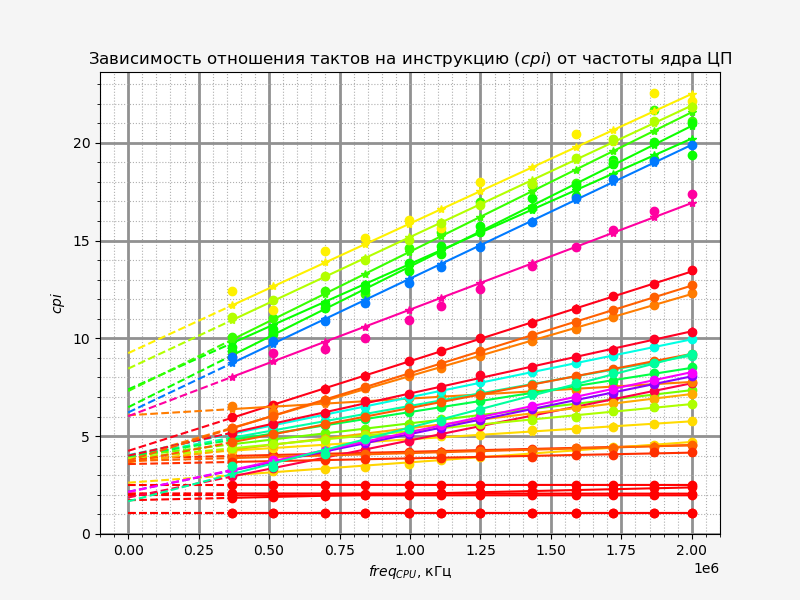
\includegraphics[width=9cm]{CPI_model.png}
        \label{pic:cpi_model}
    \end{figure}
\end{frame}

\begin{frame}{Механизмы, реализованные в ядре Linux}
    \begin{enumerate}
      \item Драйверы $clk$ и $cpufreq$ для поддержки изменения тактовых частот ядер ЦП в Gem5.
      \item Сбор статистики микроархитектурных событий для каждого ядра ЦП и потока исполнения
      в режиме реального времени и подсчёт их утилизации.
      \begin{enumerate}
          \item При смене контекста потока исполнения, ротации счётчиков
              микроархитектурных событий и по таймеру.
      \end{enumerate}
      \item Выбор тактовых частот на основе собираемой статистики
          (как по ядрам ЦП, так и по потокам исполнения).
      \begin{enumerate}
          \item При пробуждениях ядра процессора, при миграциях потоков исполнения
          на другие ядра ЦП и по таймеру.
      \end{enumerate}
      \item Политику выставления тактовых частот на основе голосования выбранных частот по ядрам ЦП.
    \end{enumerate}
\end{frame}

\section{Заключение}

\begin{frame}{Результаты и преимущества решения}
    Преимущества решения:
    \begin{enumerate}
        \item Учёт параметров, зависимых от рабочей нагрузки (кол-во обращений в ОЗУ, высокие уровни кешей).
        \item Введение параметра параллелизма обращений в память.
        \item Независимость модели от специфики работы конвейера ядра ЦП.
        \item Возможность использования в ЦП с технологией многопоточных ядер.
    \end{enumerate}

    Результаты:
    \begin{enumerate}
        \item Снижение энегопотребления синтетического приложения реального времени на 6.4\% при сохранении
        производительности.
    \end{enumerate}
\end{frame}

% =========================================

\begin{frame}
    \begin{center}
    \Huge \textcolor{faeng_blue}{Благодарю за внимание!}
    \end{center}
\end{frame}

\end{document}
